\documentclass[12pt]{article}

\usepackage[utf8]{inputenc}
\usepackage{graphicx}
\usepackage{fancyhdr}

\title{g55\_rules - Crazy Eights Legal Move Checker}
\author{Group 55\\Juliette Regimbal (260657238)\\Qingzhou Yang (260687570)}
\date{March 27, 2017}
\pagenumbering{gobble}
\pagenumbering{arabic}
\pagestyle{fancy}

\begin{document}
\maketitle
\setlength{\parindent}{0ex}
\lhead{Group 55}
\rhead{Juliette Regimbal (260657238)\\Qingzhou Yang (260687570)}
\section{Circuit Description}
The \textit{g55\_rules} circuit has two 6-bit inputs (\texttt{play\_pile\_top\_card} and \texttt{card\_to\_play}) and one 1-bit output (\texttt{legal\_play}). Based on the inputs, the circuit determines if the attempted move is legal in the game of Crazy Eights. Specifically it checks that \texttt{card\_to\_play} is a card of a value of 8, or a card of the same value as \texttt{play\_pile\_top\_card}, or a card of the same suit as \texttt{play\_pile\_top\_card}, or any suit and value if \texttt{play\_pile\_top\_card} has a value of 8. The value and suit are encoded in 6-bit unsigned integer $V$ where $V = (value - 1) + (suit * 13)$.\\

A pinout of the circuit is as follows:\\

\begin{figure}[h!t]
\centering
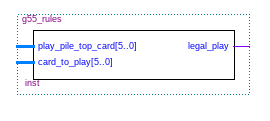
\includegraphics[scale=1.0]{graphics/rules-pinout.png}
\caption{\textit{g55\_rules} Pinout}
\end{figure}

\section{Testing}
The circuit was tested using a timing simulation. Due to the high number of possible input patters, inputs were chosen that both matched and failed each rule resulting in a true and false output respectively. The worst-case maximum propagation delay is 19.910 ns. \\

\begin{figure}[h!t]
\centering
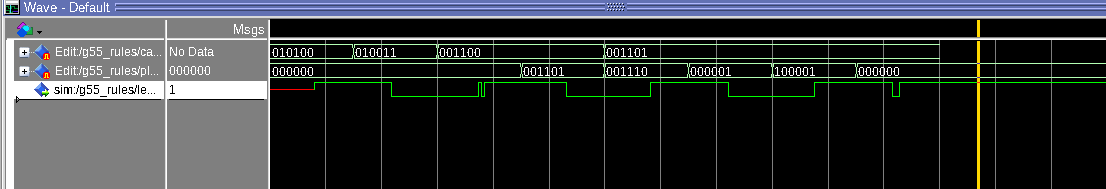
\includegraphics[scale=0.5]{graphics/rules-sim.png}
\caption{\textit{g55\_rules} Timing Simulation Results}
\end{figure}

\section{FPGA}
The \textit{g55\_rules} circuit uses a total of 40 logic elements representing less than 1\% of the total available elements on the FPGA.

\end{document}